\documentclass[journal]{IEEEtran}

\usepackage{amsmath}
\usepackage{booktabs}
\usepackage{cite}
\usepackage{graphicx}
\usepackage[hidelinks]{hyperref}
\usepackage{xcolor}

\graphicspath{{figures/}}

\newcommand{\RinexEpochCount}{3221}
\newcommand{\RinexSatelliteRowCount}{77305}
\newcommand{\DetectionRowCount}{893}
\newcommand{\RinexCoverageRows}{893}
\newcommand{\AttackPrecision}{0.382}
\newcommand{\AttackRecall}{0.950}
\newcommand{\AttackFone}{0.545}
\newcommand{\AttackRocAuc}{0.951}
\newcommand{\AttackLatencyMean}{2.000}
\newcommand{\BestFoneThreshold}{1.249}
\newcommand{\BestFonePrecision}{0.592}
\newcommand{\BestFoneRecall}{0.925}
\newcommand{\BestFoneScore}{0.722}
\newcommand{\CleanFalseAlarmPerMinute}{9.474}
\newcommand{\RinexMeanSatellites}{24.00}
\newcommand{\RawRaimCoverageRows}{47}
\newcommand{\RawRaimDetectedRows}{3}
\newcommand{\RawReferenceResidualMean}{0.734}
\newcommand{\MatrixScenarioCount}{82}
\newcommand{\MatrixAttackScenarioCount}{80}
\newcommand{\AdaptiveSeqPrecision}{0.513}
\newcommand{\AdaptiveSeqRecall}{0.520}
\newcommand{\AdaptiveSeqFone}{0.464}
\newcommand{\AdaptiveSeqLatency}{32.937}
\newcommand{\AdaptiveSeqCleanFalseAlarm}{5.510}
\newcommand{\AdaptiveSeqFalseAlarm}{2.788}
\newcommand{\AdaptiveSeqDegradedFalseAlarm}{0.067}
\newcommand{\FixedFusedMatrixFone}{0.365}
\newcommand{\FixedFusedPrecision}{0.509}
\newcommand{\FixedFusedRecall}{0.301}
\newcommand{\FixedFusedCleanFalseAlarm}{5.241}
\newcommand{\FixedFusedDegradedFalseAlarm}{7.189}
\newcommand{\FixedFusedMatrixFalseAlarm}{6.215}
\newcommand{\PseudorangeGlrtFone}{0.386}
\newcommand{\PseudorangeGlrtPrecision}{0.459}
\newcommand{\PseudorangeGlrtRecall}{0.369}
\newcommand{\PseudorangeGlrtFalseAlarm}{5.375}
\newcommand{\LioResidualFone}{0.357}
\newcommand{\LioResidualPrecision}{0.221}
\newcommand{\LioResidualRecall}{0.932}
\newcommand{\LioResidualFalseAlarm}{58.658}
\newcommand{\RaimOnlyFone}{0.013}
\newcommand{\RaimOnlyPrecision}{0.050}
\newcommand{\RaimOnlyRecall}{0.008}
\newcommand{\AdaptiveFusedFone}{0.188}
\newcommand{\AdaptiveFusedPrecision}{0.693}
\newcommand{\AdaptiveFusedRecall}{0.111}
\newcommand{\AdaptiveFusedFalseAlarm}{1.008}
\newcommand{\NoRawFone}{0.093}
\newcommand{\NoLioFone}{0.025}
\newcommand{\NoEnvFone}{0.306}
\newcommand{\NoCusumFone}{0.188}
\newcommand{\AttackTypeBestName}{position bias}
\newcommand{\AttackTypeBestFone}{0.491}
\newcommand{\AttackTypeWorstName}{slow drift}
\newcommand{\AttackTypeWorstFone}{0.421}
\newcommand{\AttackTypeWorstRecall}{0.406}
\newcommand{\AttackClassificationDominantFraction}{0.848}
\newcommand{\SensitivityBestFone}{0.473}
\newcommand{\SensitivityBestGain}{1.35}
\newcommand{\SensitivityBestCusum}{0.35}
\newcommand{\SensitivitySelectedFone}{0.464}
\newcommand{\SensitivitySelectedFalseAlarm}{2.788}
\newcommand{\AdaptiveVsFixedFoneGain}{0.099}
\newcommand{\AdaptiveVsFixedCiLow}{0.046}
\newcommand{\AdaptiveVsFixedCiHigh}{0.146}
\newcommand{\AdaptiveVsFixedPvalue}{0.0002}


\title{Toward Robust GNSS Spoofing Detection with Raw Observation and LiDAR--Inertial Consistency}

\author{Zhibo Wang%
\thanks{This draft is generated from the reproducible C++/Python GNSS spoof-detection platform in this repository.}}

\begin{document}
\maketitle

\begin{abstract}
GNSS spoofing can induce hazardous navigation errors while preserving apparently plausible satellite measurements.
This paper presents a reproducible spoofing-detection platform that combines raw RINEX observation features, RTKLIB solution products, and LiDAR--inertial consistency diagnostics from FAST\_GLIO.
The platform converts GPS time and Unix time onto a common axis, extracts per-satellite code, carrier, signal-strength, and loss-of-lock features, injects controlled synthetic spoofing windows, and reports precision, recall, F1 score, ROC AUC, false-alarm rate, and detection latency.
On the current rover dataset, the RINEX extractor produces \RinexEpochCount{} epochs and \RinexSatelliteRowCount{} per-satellite observation rows, all of which are synchronized into the \DetectionRowCount{}-sample detection dataset.
The first transparent baseline achieves recall \AttackRecall{} and ROC AUC \AttackRocAuc{} under synthetic spoofing, exposing the need for environment-adaptive gates and raw-observation residual tests in the next stage.
\end{abstract}

\begin{IEEEkeywords}
GNSS spoofing detection, RINEX, LiDAR--inertial odometry, RTKLIB, FAST\_GLIO, raw observation consistency.
\end{IEEEkeywords}

\section{Introduction}
Civil GNSS receivers are widely used in robotic, aerial, and ground navigation systems.
Their open signal structure, however, makes them vulnerable to spoofing attacks that can bias the estimated position without immediately causing signal loss.
Classical receiver-side residual tests can detect abrupt faults, but benign degradation caused by multipath, occlusion, and poor satellite geometry can look similar to adversarial behavior.
This motivates a multi-source detection strategy that compares raw GNSS consistency with an independent LiDAR--inertial motion estimate.

This paper develops a reproducible platform for GNSS spoofing studies.
Rather than treating post-fusion trajectory errors as the only signal, the platform preserves raw observation features, RTK quality indicators, DOP values, pseudorange residual diagnostics, and LiDAR--GNSS consistency residuals.
The long-term objective is a publishable detector that separates spoofing from ordinary degradation with low false-alarm rate and short detection latency.

The current contributions are:
\begin{itemize}
    \item a C++/Python experiment platform that links flight simulation, RINEX observations, RTKLIB products, FAST\_GLIO logs, and visualization;
    \item a RINEX feature extractor that outputs both per-satellite long-format observations and per-epoch summaries;
    \item a synchronized detection dataset that merges raw observation quality, RTK/DOP, raw GNSS update diagnostics, and LiDAR--inertial consistency;
    \item a first transparent baseline with reproducible metrics and figures.
\end{itemize}

\section{Related Work}
GNSS spoofing detection methods can be broadly grouped into signal-level monitoring, measurement-level residual tests, navigation filter innovation tests, and cross-modal consistency checks.
Signal-level approaches can be powerful but often require tracking-channel access or specialized antennas.
Measurement-level approaches such as RAIM and GLRT are deployable on receiver outputs, but they can be sensitive to multipath and satellite geometry.
Cross-modal approaches compare GNSS with inertial, visual, LiDAR, wheel odometry, or map constraints.
This work focuses on a deployable measurement/navigation-layer platform that uses RINEX raw observations~\cite{rinex304}, RTKLIB products~\cite{rtklib}, and LiDAR--inertial consistency inspired by FAST-LIO2~\cite{fastlio2} without custom RF hardware.

\section{System Overview}
Fig.~\ref{fig:architecture} shows the implemented pipeline.
The platform ingests RINEX observation files, RTKLIB solution products, FAST\_GLIO fusion diagnostics, and C++ simulator outputs.
All data streams are aligned to Unix time, with GPS time converted using an explicit GPST--UTC offset.
The detector consumes a single synchronized table that preserves raw GNSS quality, RTK quality, DOP, pseudorange residual statistics, and LiDAR--GNSS residuals.

\begin{figure}[!t]
    \centering
    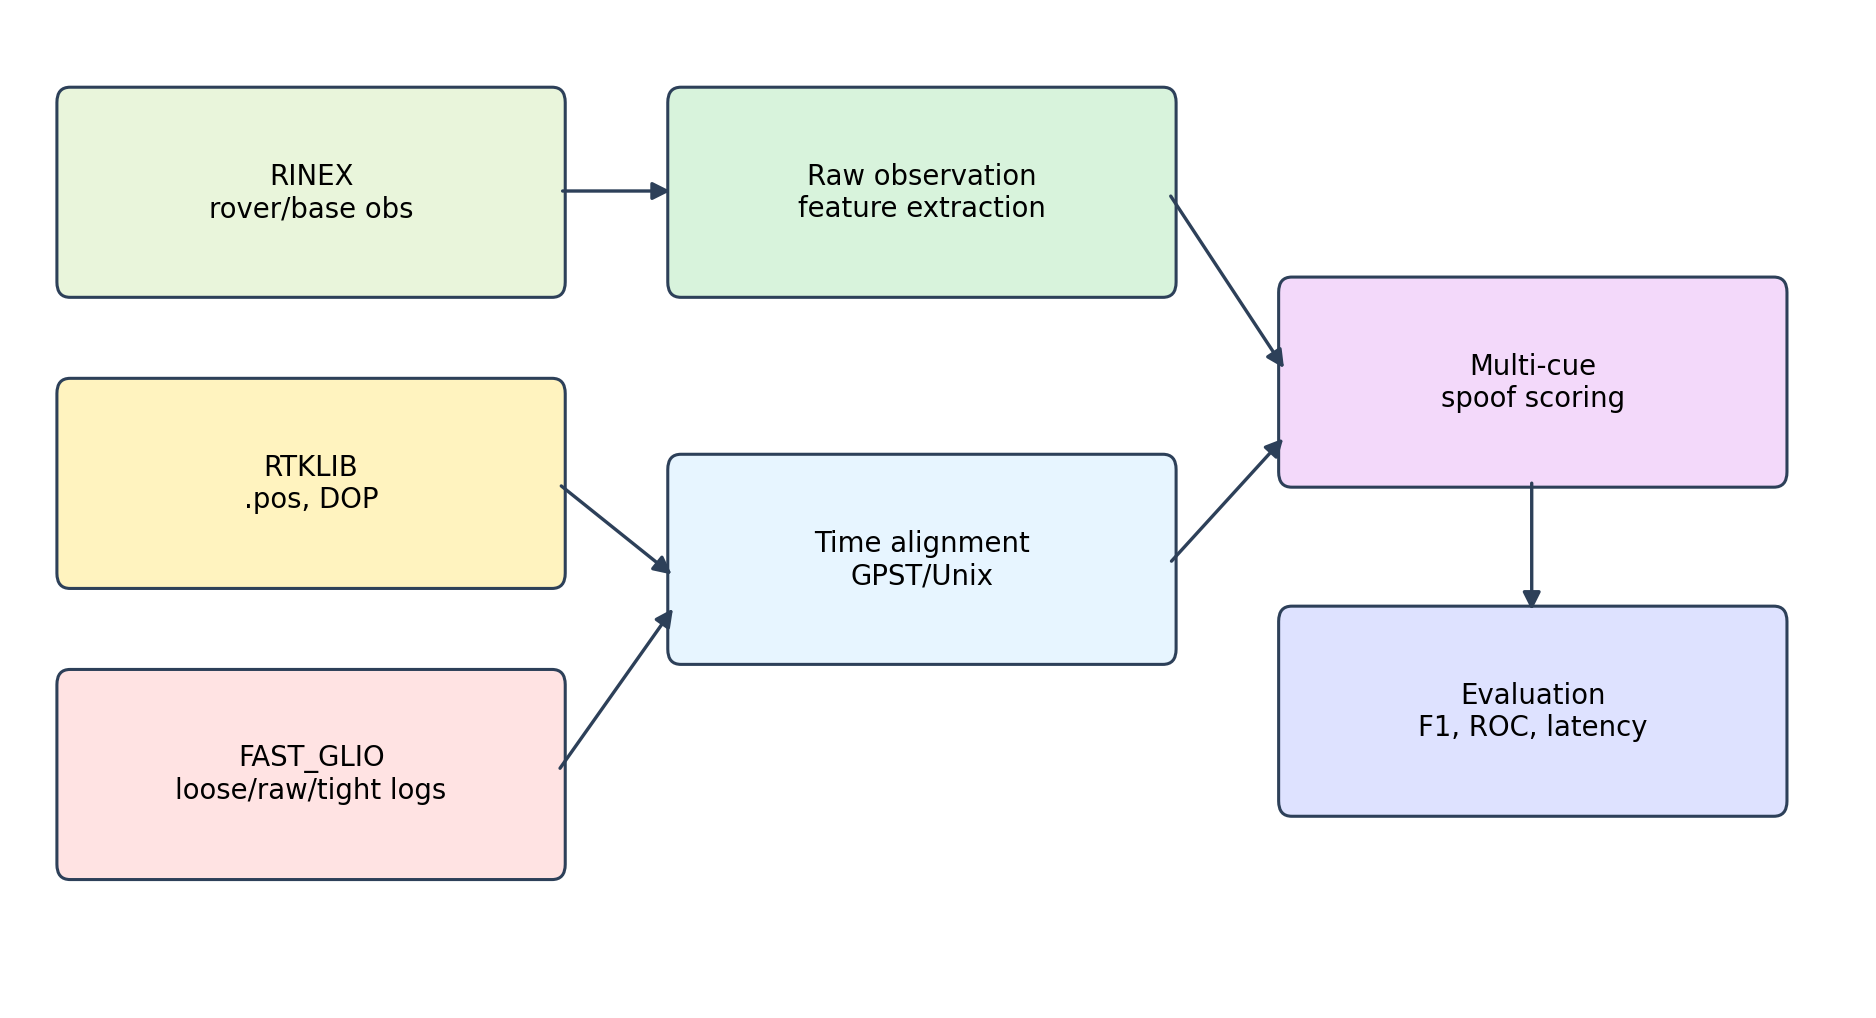
\includegraphics[width=\linewidth]{system_architecture.png}
    \caption{Reproducible platform architecture. RINEX, RTKLIB, and FAST\_GLIO products are synchronized before multi-cue spoof scoring and evaluation.}
    \label{fig:architecture}
\end{figure}

\section{Raw Observation Feature Extraction}
The RINEX parser reads the system-specific observation type declarations and decodes each satellite record into code, carrier, Doppler when present, C/N0, LLI, and SSI fields.
It outputs a per-satellite table with one row per satellite per epoch and a per-epoch summary with satellite count, constellation coverage, observation counts, C/N0 statistics, inter-frequency code-difference RMS, and loss-of-lock counts.
The current rover observation file contains an average of \RinexMeanSatellites{} satellites per epoch.

Fig.~\ref{fig:rawobs} summarizes the raw observation stream.
The rover RINEX file contains GPS, GLONASS, Galileo, BeiDou, QZSS, and IRNSS observations.
The current rover file does not expose Doppler observation types, so Doppler/TDCP residuals remain a next-step feature for the rover stream; the extraction code supports Doppler fields when present, as in the base observation file.

\begin{figure}[!t]
    \centering
    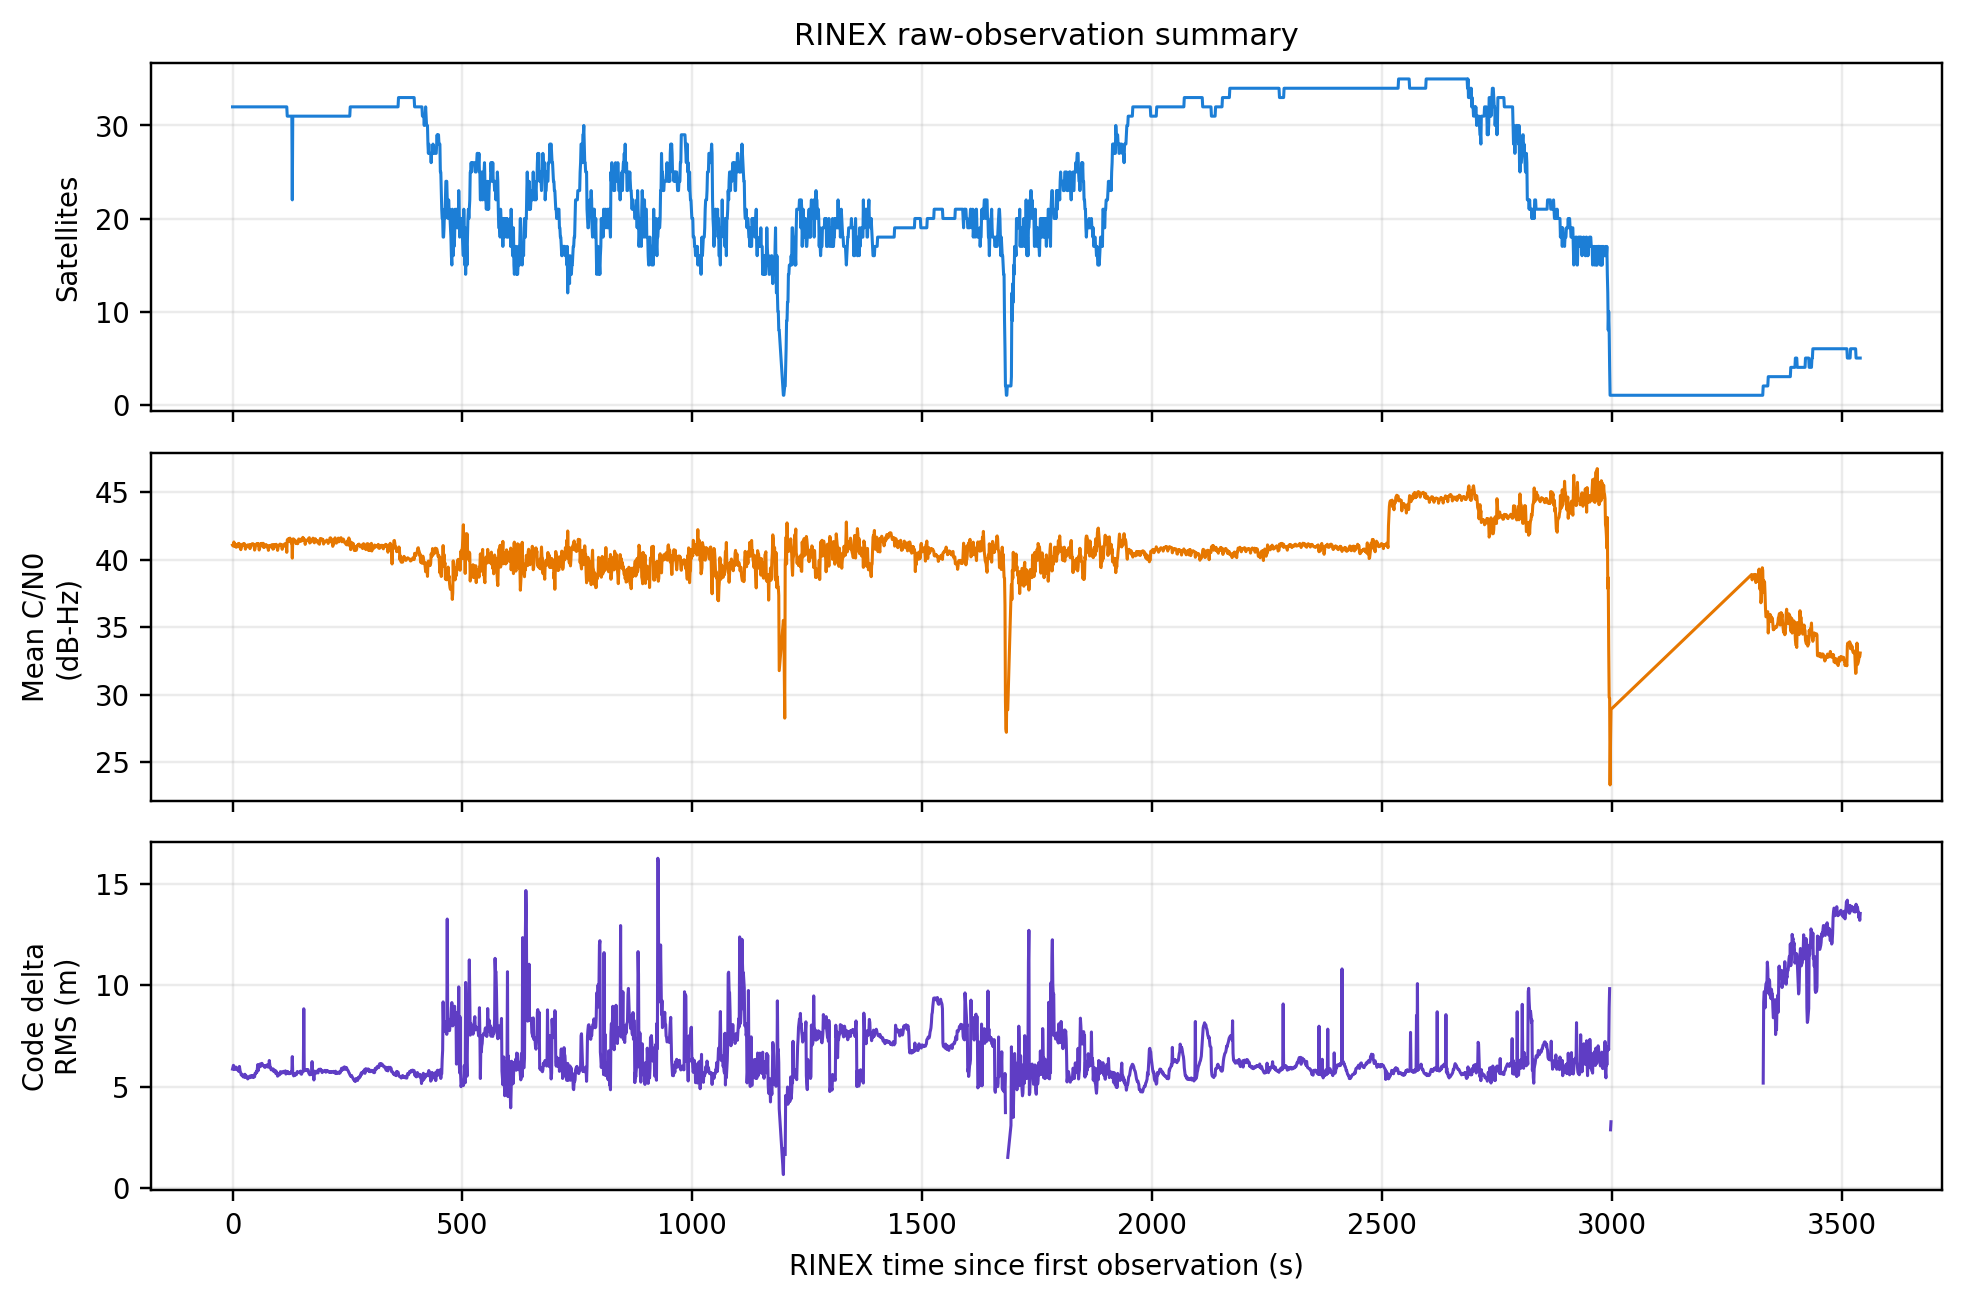
\includegraphics[width=\linewidth]{raw_observation_summary.png}
    \caption{RINEX raw-observation summary: satellite count, mean C/N0, and inter-frequency code-difference RMS over the rover observation interval.}
    \label{fig:rawobs}
\end{figure}

\begin{figure}[!t]
    \centering
    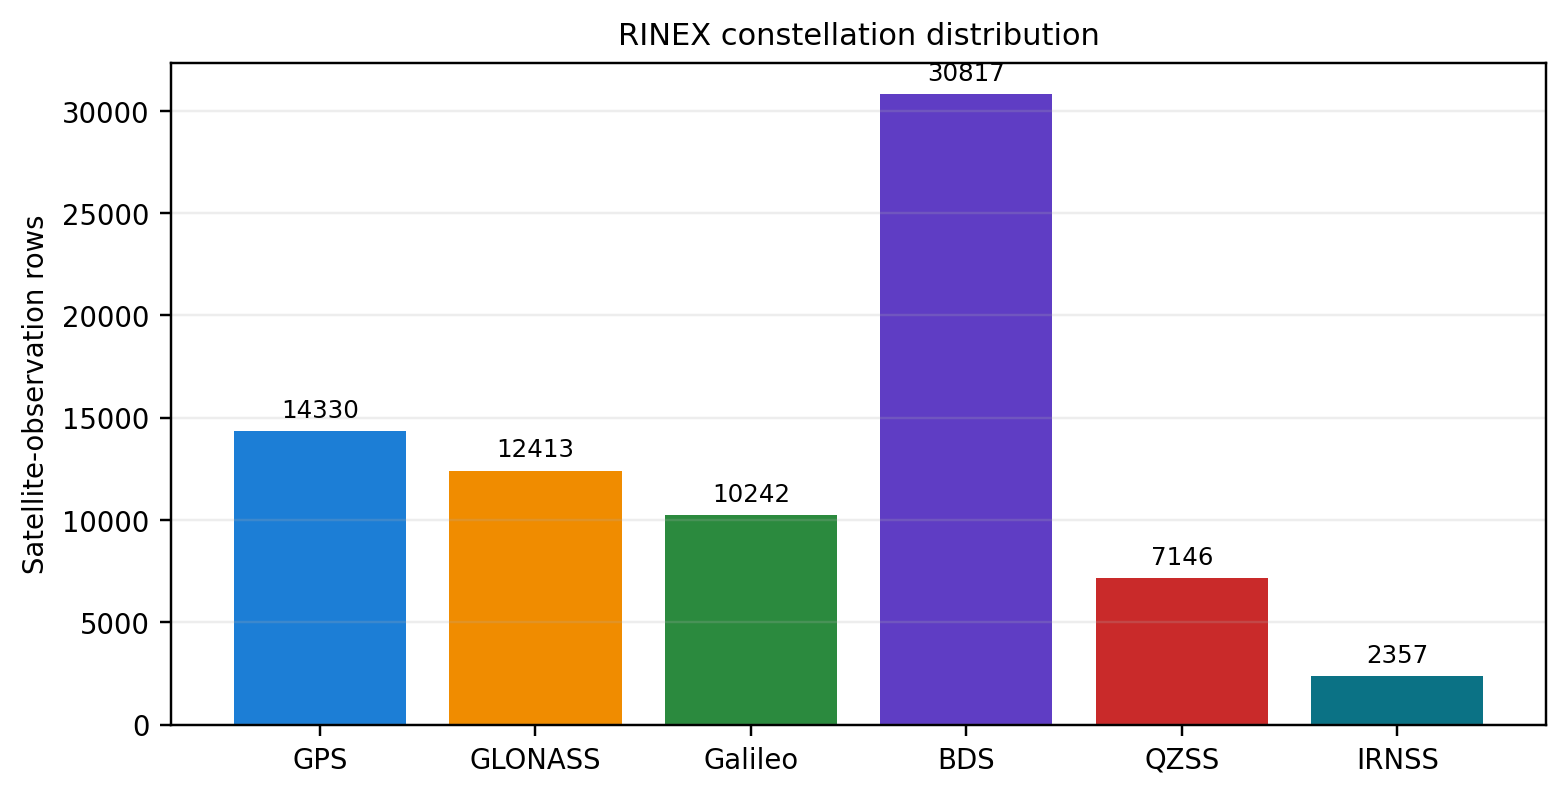
\includegraphics[width=\linewidth]{constellation_distribution.png}
    \caption{Constellation distribution in the rover RINEX file, counted over per-satellite observation rows.}
    \label{fig:constellation}
\end{figure}

\section{Detection Dataset and Baseline}
The synchronized detection table currently contains \DetectionRowCount{} samples.
The RINEX epoch summary covers \RinexCoverageRows{} of these samples.
Each row includes the spoofing label, detector output, score components, RTK quality, DOP, FAST\_GLIO raw pseudorange diagnostics, LiDAR--GNSS residuals, and RINEX raw-observation summaries.

The baseline spoofing score is a weighted sum of normalized terms:
\begin{equation}
S =
w_r S_r + w_m S_m + w_p S_p + w_a S_a + w_d S_d + w_q S_q ,
\end{equation}
where $S_r$ is the LiDAR--GNSS residual score, $S_m$ is the Mahalanobis gate score, $S_p$ and $S_a$ are pseudorange RMS and maximum-residual scores, $S_d$ is the Doppler/TDCP score when available, and $S_q$ penalizes degraded RTK quality.
The detector triggers when $S$ exceeds a threshold and confirms spoofing after a configurable number of consecutive triggered samples.

Fig.~\ref{fig:trajectory} shows the real RTK route and raw-observation availability.
Fig.~\ref{fig:score} shows the synthetic spoofing interval and baseline score response.

\begin{figure}[!t]
    \centering
    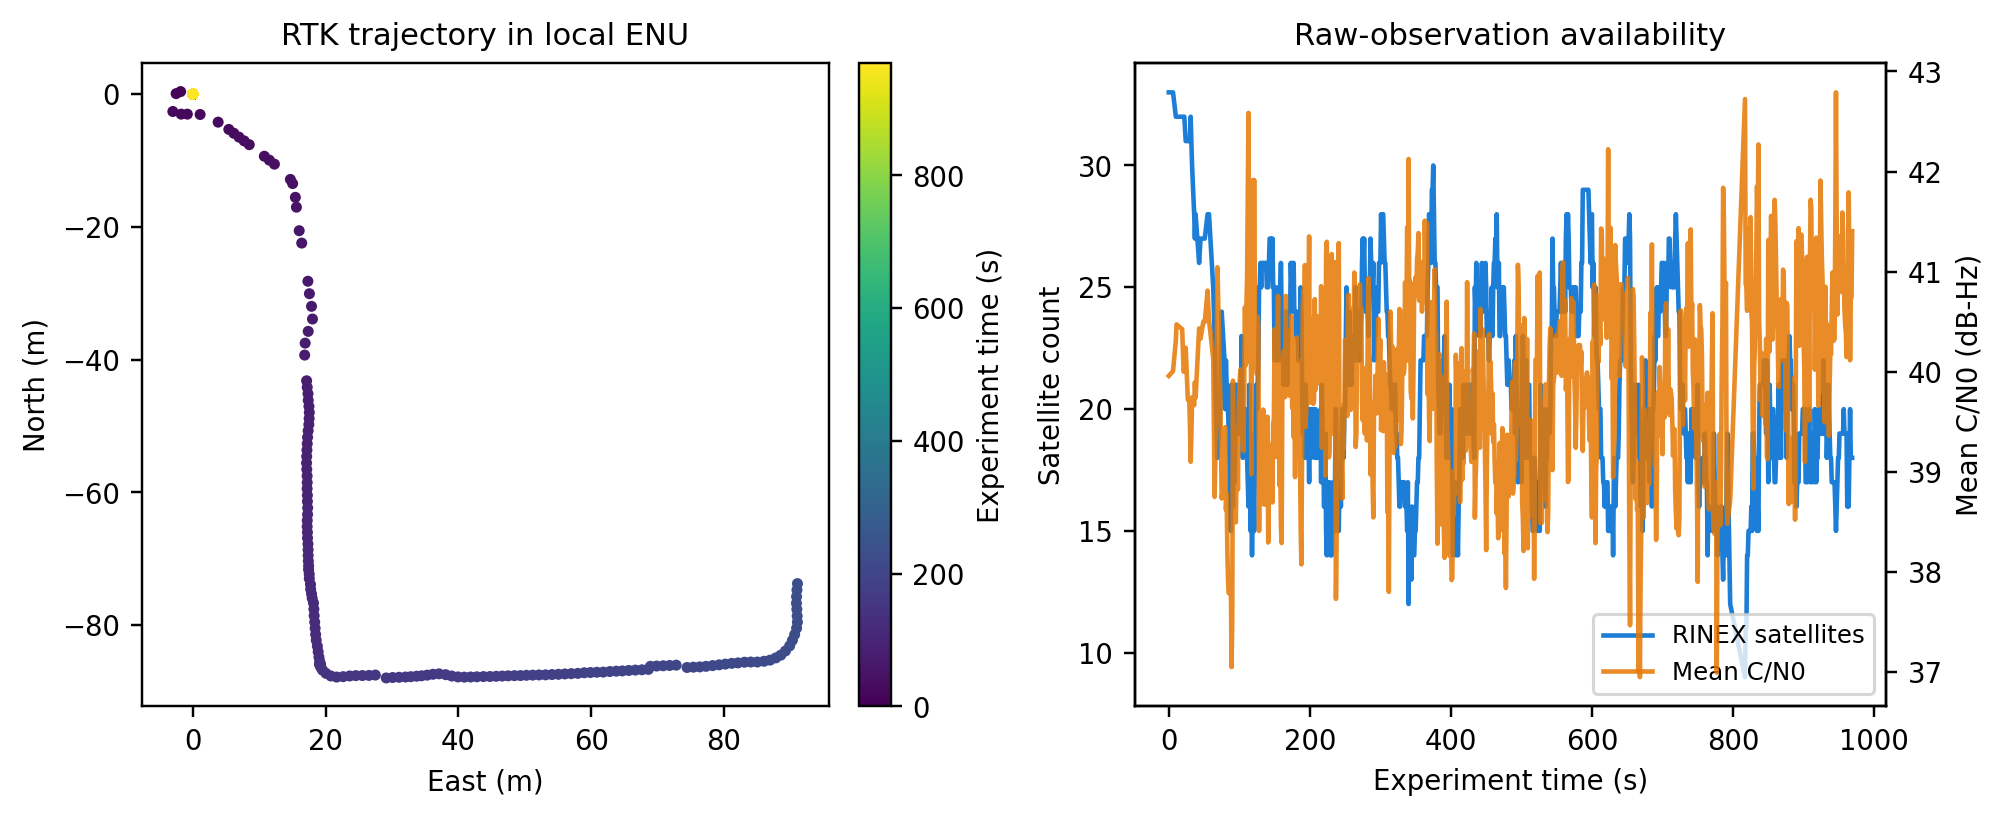
\includegraphics[width=\linewidth]{trajectory_quality.png}
    \caption{RTK trajectory and synchronized RINEX observation availability.}
    \label{fig:trajectory}
\end{figure}

\begin{figure}[!t]
    \centering
    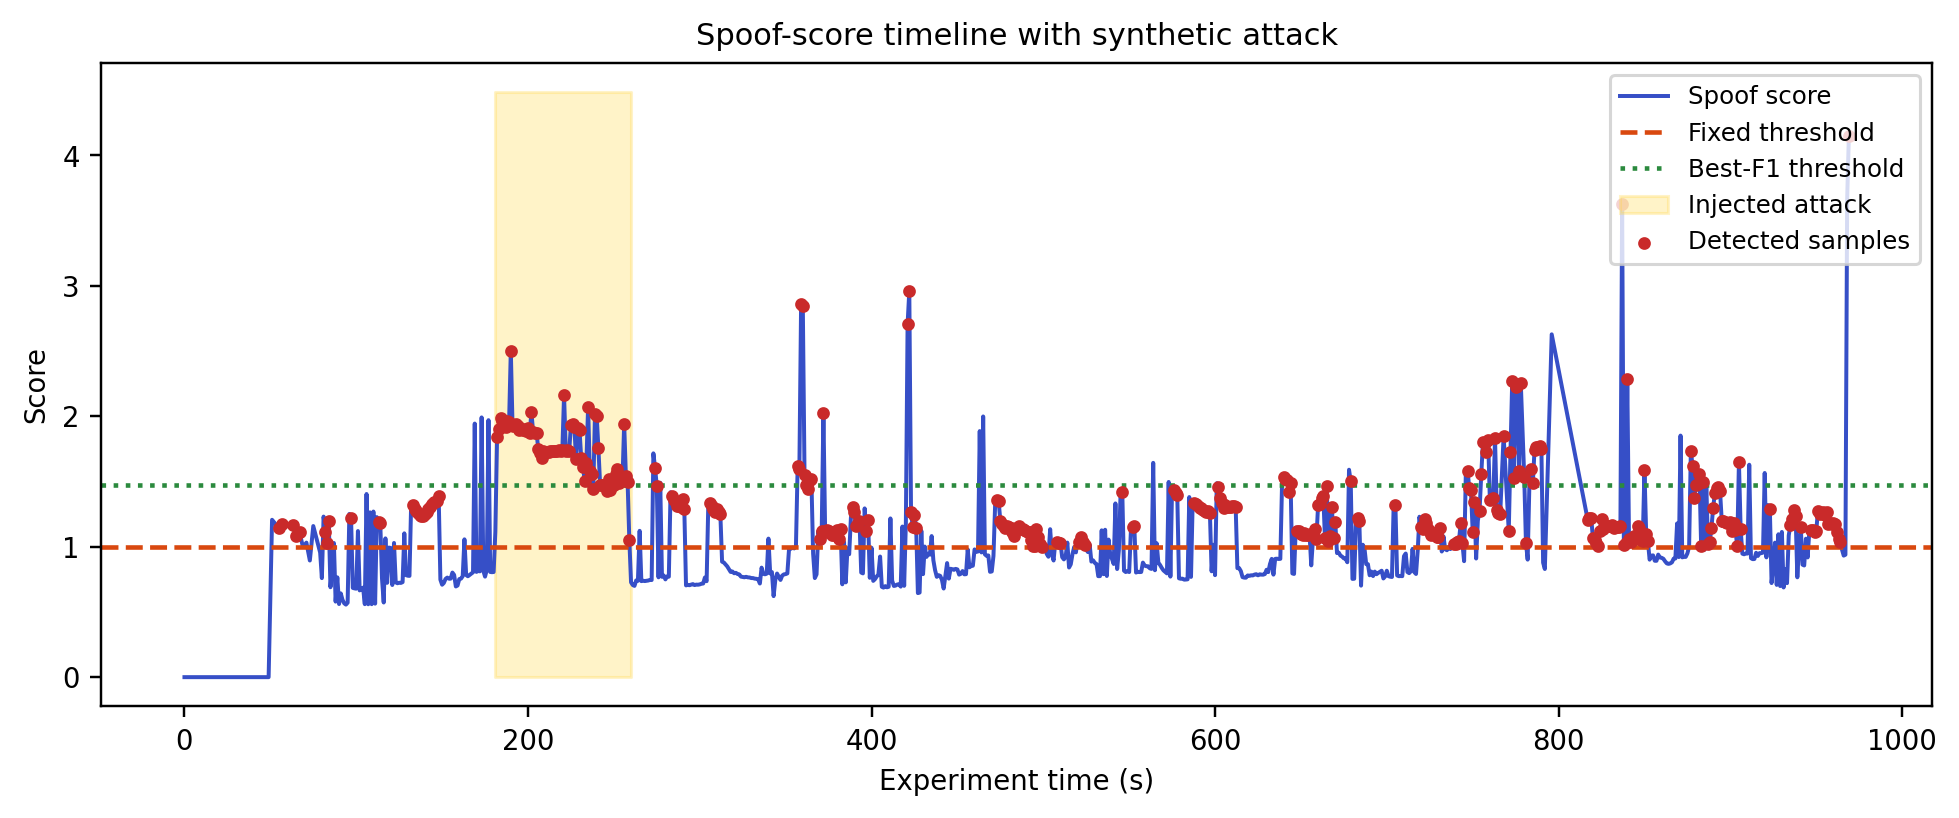
\includegraphics[width=\linewidth]{spoof_score_timeline.png}
    \caption{Spoof-score timeline for the synthetic attack case. The baseline fixed threshold detects the attack but also produces false alarms in degraded clean intervals.}
    \label{fig:score}
\end{figure}

\section{Preliminary Results}
Table~\ref{tab:metrics} reports the current baseline on the synthetic spoofing run.
The fixed-threshold detector reaches high recall but low precision, which confirms that static thresholds are too sensitive for this dataset.
Threshold calibration improves F1 from \AttackFone{} to \BestFoneScore{}, with threshold \BestFoneThreshold{}.

\begin{table}[!t]
\centering
\caption{Preliminary synthetic-spoofing metrics.}
\label{tab:metrics}
\begin{tabular}{lc}
\toprule
Metric & Value \\
\midrule
Fixed-threshold precision & \AttackPrecision{} \\
Fixed-threshold recall & \AttackRecall{} \\
Fixed-threshold F1 & \AttackFone{} \\
ROC AUC & \AttackRocAuc{} \\
Mean detection latency (s) & \AttackLatencyMean{} \\
Best-F1 threshold & \BestFoneThreshold{} \\
Best-F1 precision & \BestFonePrecision{} \\
Best-F1 recall & \BestFoneRecall{} \\
Best-F1 score & \BestFoneScore{} \\
Clean false alarms/min & \CleanFalseAlarmPerMinute{} \\
\bottomrule
\end{tabular}
\end{table}

\begin{figure}[!t]
    \centering
    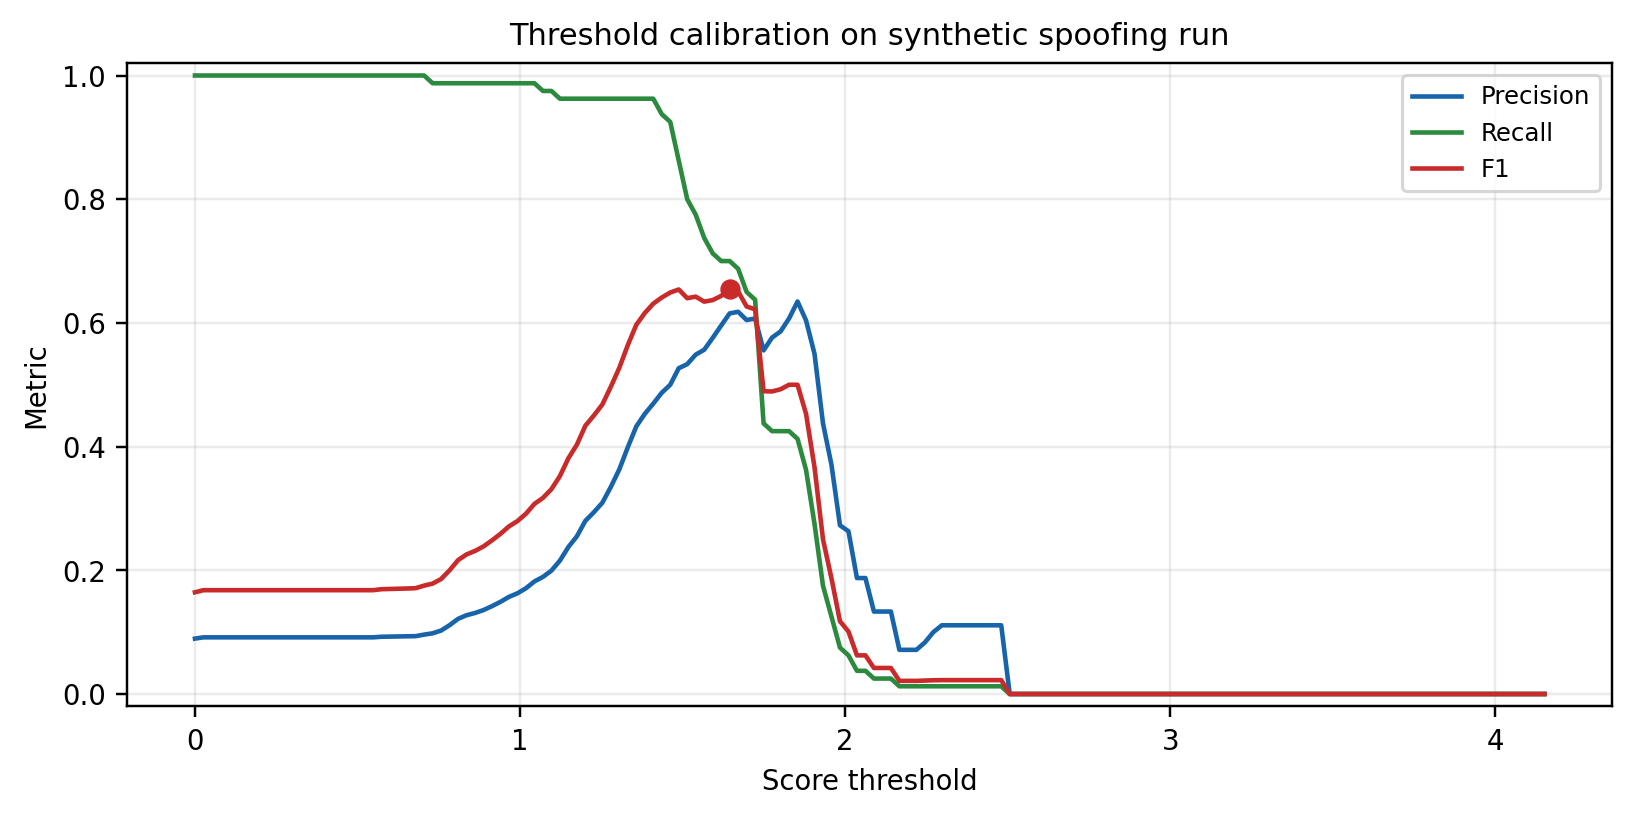
\includegraphics[width=\linewidth]{threshold_calibration.png}
    \caption{Threshold calibration for the synthetic spoofing run. The current fixed threshold is intentionally transparent but not yet publication quality.}
    \label{fig:threshold}
\end{figure}

\section{Next Steps Toward a Journal Paper}
The next research stage should move from residual-level injection to raw-observation-level attack modeling.
Specifically, we will estimate satellite geometry from navigation ephemerides, compute predicted pseudorange and Doppler/TDCP residuals, and implement RAIM-only, LiDAR--GNSS-only, raw-GNSS-only, and fused adaptive baselines.
The main algorithmic opportunity is an environment-aware sequential detector that adapts thresholds using C/N0, DOP, constellation coverage, LIO quality, and RTK ambiguity indicators.
This is also where the platform can turn the current false-alarm weakness into a publishable contribution.

\section{Conclusion}
This draft presents a reproducible GNSS spoofing-detection platform with raw RINEX observation features and LiDAR--inertial consistency diagnostics.
The first experimental figures and metrics are generated directly from the repository pipeline.
The results show that the data path is now ready for raw residual modeling, adaptive gating, and systematic ablation studies.

\bibliographystyle{IEEEtran}
\bibliography{references}

\end{document}
